\documentclass[11pt,a4paper]{article}
\usepackage[margin=1in, headheight=14pt]{geometry}
\usepackage{amsfonts,amsmath,amssymb,suetterl}
\usepackage{lmodern}
\usepackage[T1]{fontenc}
\usepackage{fancyhdr}
\usepackage{float}
\usepackage[utf8]{inputenc}
\usepackage{fontawesome}
\usepackage{enumerate}
\usepackage{xcolor}
\usepackage{hyperref}
\usepackage{mathtools}
\usepackage{tikz}

\DeclareUnicodeCharacter{2212}{-}

\usepackage{mathrsfs}
\usepackage[nodisplayskipstretch]{setspace}

\setstretch{1.5}
\renewcommand{\footrulewidth}{0pt}

\parindent 0ex
\setlength{\parskip}{1em}
\pagestyle{empty}

\begin{document}
    %
	\begin{singlespace}
		\begin{center}
			\Huge Queen Mary\\
			\LARGE University of London
		\end{center}
		\Large \textbf{MTH5123} \hfill \Large \textbf{Differential Equations,} \hfill \Large \textbf{Fall 2020}\\
		\large \textbf{Coursework 4 week 8 - Solutions} \hfill \large \textbf{W. Huang}
		\rule{\textwidth}{0.4pt}
	\end{singlespace}
	%
	\textbf{I. Practice Problems}\par
	\textbf{Correction: all coordinates should be $y_1, y_2$ plane, instead of $xy$ plane in all figures.}
	%
	\begin{enumerate}[\bfseries A.]
		\item Sketch the following parametric curves:
		\begin{enumerate}[\bfseries 1)]
			\item $
			\begin{dcases}
				y_1(t) = t + 1\\
				y_2(t) = 2t − 3
			\end{dcases}\quad
			\text{for $0 \leq t < \infty$.}
			$
			\textbf{Solution:} Using the first equation to eliminate the parameter, we obtain the equation of the line $y_2 = 2y_1 − 5$. To determine the direction of the parametric curve, by examining various values of $t$, for example, we see that the arrow on this line points from the third quadrant to the first quadrant.
			%
			\begin{figure}[H]
				\centering
					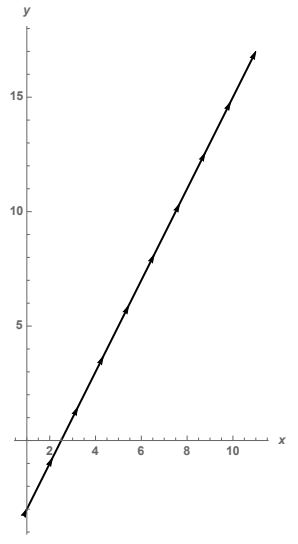
\includegraphics[width=0.35\textwidth]{figure/figA1.PNG}
			\end{figure}
			%
			\item $
			\begin{dcases}
				y_1(t) = t^2 - 1\\
				y_2(t) = 4t + 3
			\end{dcases}\quad
			\text{for $0 \leq t < \infty$.}
			$
			\textbf{Solution:} Using the second equation to eliminate the parameter, we obtain the equation of a parabolaUsing the second equation to eliminate the parameter, we obtain the equation of a parabola $y_1 = \frac{1}{16}(y_2-1)^2-1$, which opens to the right and has vertex $(−1, 1)$ and crosses the $y_2$-axis at $\pm 5$. To graph the parametric curve for $0 \leq t \leq \infty$, we find $(y_1(0), y_2(0)) = (−1, 1)$ and for $t > 0$, we follow the upper branch of this parabola to infinity.
			%
			\begin{figure}[H]
				\centering
					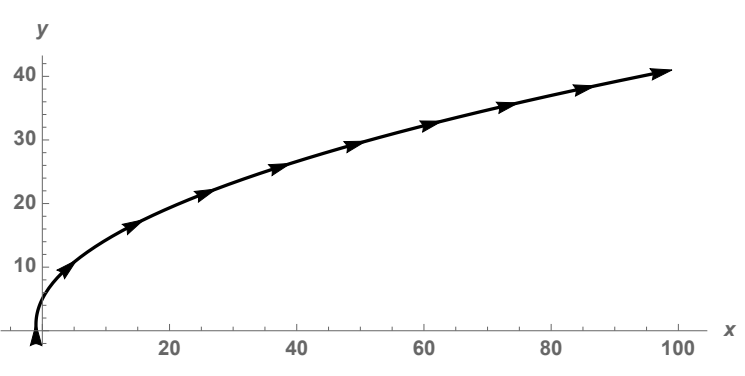
\includegraphics[width=0.55\textwidth]{figure/figA2.PNG}
			\end{figure}
			%
			\item $
			\begin{dcases}
				y_1(t) = 5\cos t\\
				y_2(t) = 4\sin t
			\end{dcases}\quad
			\text{for $0 \leq t \leq 4\pi$.}
			$
			\textbf{Solution:}  Here, we observe that $y_1/5 = \cos t$ and $y_2/4 = \sin t$, combined with the fact that $\sin^2t + \cos^2t=1$, we have the equation of an ellipse centred at the origin: $(\frac{y_1}{5})^2+(\frac{y_2}{4})^2 = 1$, and crossing the $y_1$-axis at $\pm 5$ and the $y_2$-axis at $\pm 4$. The direction of the arrow for the parametric curve is anticlockwise (try $t = 0,\ \pi/2,\ \pi,\ \ldots$). The parametric curve starts at $(y_1(0),\ y_2(0)) = (5, 0)$ and goes around the ellipse twice before ending at the same point.
			%
			\begin{figure}[H]
				\centering
					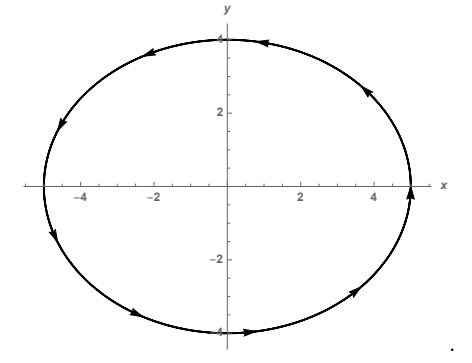
\includegraphics[width=0.5\textwidth]{figure/figA3.PNG}
			\end{figure}
			%
		\end{enumerate}
		\item Compute all equilibria of the following ODE systems
		\begin{enumerate}[\bfseries 1)]
			\item $$
			\dot{y_1} = y_1^2 - 4y_2,\quad \dot{y_2} = (y_1+2)y_2.
			$$
			\textbf{Solution:} The equilibria can be found when $\dot{y_1} = 0$ and $\dot{y_2} = 0$. There are in total 2 equilibria of this ODE system. The right-hand side $\dot{y_2} = (x+2)y2 = 0$ for either $y_1 = −2$ or $y_2 = 0$. For $y_1 = −2$ the right-hand side $\dot{y_1} = y_1^2 - 4y_2 = 0$ vanishes for $y_2 = 1$, hence we have an equilibrium at the point $(−2, 1)$ in the $(x, y)$ plane. For $y_2 = 0$ the right-hand side $\dot{y_1} = y_1^2 - 4y_2$ for $y_1 = y_2 = 0$, which responds to the other equilibrium at the point $(0, 0)$.
			\item $$
			\dot{y_1} = y_2^2+y_1y_2,\quad \dot{y_2} = y_1^2-2y_2-5y_1+2.
			$$
			\textbf{Solution:} The equilibria can be found when $\dot{y_1} = 0$ and $\dot{y_2} = 0$. There are in total 4 equilibria of this ODE system. The right-hand side $\dot{y_1} = y_2^2+y_1y_2 = 0$. For $y_1 = y_2$ the right-hand side $\dot{y_2} = y_1^2-2y_2-5y_1+2 = y_1^2-3y_1+2 = (y_1-1)(y_1-2) = 0$ for $y_1 = 1$ or $y_1 = 2$, hence we have two equilibria at the points $(1, −1)$ and $(2, −2)$ in the $(y_1, y_2)$ plane. For $y_2 = 0$ the right-hand side $\dot{y_1} = y_1^2-5y_1 + 2 =0$ for $y_1 = \frac{5-\sqrt{17}}{2}$ and $y_1 = \frac{5+\sqrt{17}}{2}$, which responds to the other two equilibria at the points, $(\frac{5-\sqrt{17}}{2}, 0)$ and $(\frac{5+\sqrt{17}}{2}, 0)$.
		\end{enumerate}
		\item  In this exercise we practice graphing parametric curves in both cartesian and polar coordinates.
		\begin{enumerate}[\bfseries 1)]
			\item  Graph the parametric curve given by
			$
			\begin{dcases}
				y_1(t) = e^{-t}\sin 3t\\
				y_2(t) = e^{-t}\cos 3t
			\end{dcases}\quad
			\text{for $0 \leq t < \infty$}.
			$
			\item Graph the curve defined by the function $r = 4 \sin \theta$ in the cartesian coordinate. Hint: Multiply both sides by $r$ and use the transformation $y_1 = r \cos \theta,\ y_2 = r \sin \theta$ to rewrite the equation in Cartesian coordinates $(y_1, y_2)$.
			\item Graph $r = \theta$ in the cartesian coordinate. Write 1-2 sentences comparing the graphs of 1) and 3).
		\end{enumerate}
		\textbf{Solution:}
		\begin{enumerate}[\bfseries 1)]
			\item $y_1(t) = e^{-t}\sin 3t,\ y_2(t) = e^{-t}\cos 3t$, for $0 \leq t < \infty$ is a clockwise spiral, starting at $(0,1)$, circling toward the origin.
			%
			\begin{figure}[H]
				\centering
					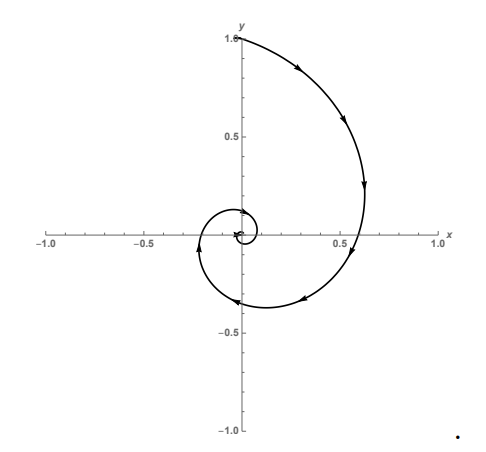
\includegraphics[width=0.40\textwidth]{figure/figC1.PNG}
			\end{figure}
			\begin{figure}[H]
				\centering
					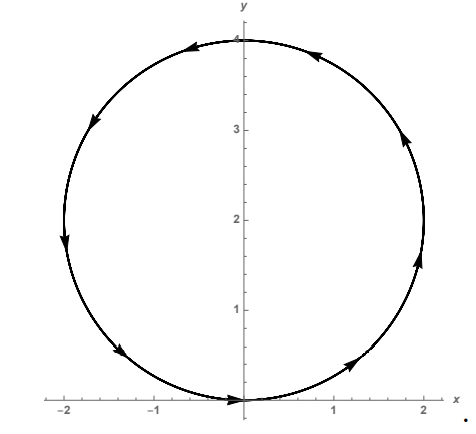
\includegraphics[width=0.40\textwidth]{figure/figC2.PNG}
			\end{figure}
			%
			\item  Using the transformation $y_1 = r \cos \theta,\ y_2 = r \sin \theta$, and multiplying $r = 4 \sin \theta$ by $r$, gives $r^2 = 4r\sin \theta\ \Leftrightarrow\ r^2(\cos^2\theta + \sin^2\theta) = 4(r\sin \theta)\ \Leftrightarrow\ y_1^2 + y_2^2 = 4y$. Rearranging the terms, we have $y_1^2 + (y_2-2)^2=4$, which is a circle centred at $(0, 2)$ of radius $2$. The parametric curve traverses this curve anticlockwise.
			\item Using the transformation $y_1 = r \cos \theta,\ y_2 = r \sin \theta$ and $r = \theta$, thus $y_1 = \theta \cos \theta,\ y_2 = \theta \sin \theta$ and $_1^2+y_2^2 = \theta^2$. When $\theta = 0$, the parametric curve is at the origin of the  Cartesian coordinates $(y_1, y_2)$. When $\theta = 0,\ \pi,\ 2\pi,\ \ldots$, it hits the $x$ coordinate. When $\theta = \frac{}{2}\pi,\ \frac{3}{2}\pi,\ \ldots$, it hits the $y$ coordinate. The value of $\sqrt{y_1^2 + y_2^2}$, which is also the distance between the point where the parametric curve hits the $x$ or $y$ coordinate and the origin, linearly increases with $\theta$ because $y_1^2 + y_2^2 = \theta^2$. Thus, we can plot this parametric curve as an outward anticlockwise spiral starting at the origin.
			%
			\begin{figure}[H]
				\centering
					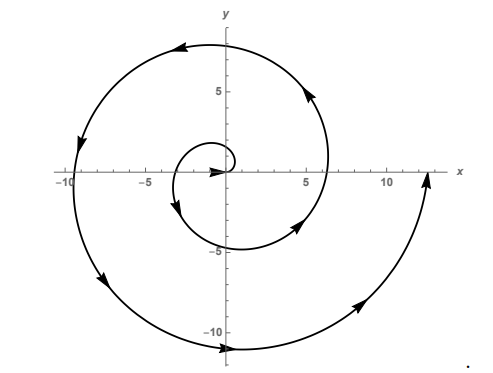
\includegraphics[width=0.40\textwidth]{figure/figC3.PNG}
			\end{figure}
			%
			Comparing the graphs in (1) and (3), we can see that graph 1) is spiral into the origin, and graph 3) is spiral away from the origin. (Why? This is because the coefficient function before sin and cos are different in these two questions. In (1), it is $e^{-t}$ which decreases with $t$, and in (3) is $\theta$ which linearly increases with $\theta$. This is relevant to our week 9-10 lectures.)
		\end{enumerate}
		\item In week 1 lecture, we learned the logistic equation, which is an application of using first order ODE in biology to model population growth (see our typed lecture notes and Video week 1 session 1-2 if you are not familiar with this example). In this model, the change of population size over time is governed by a 1st-order non-linear separable differential equation.
		$$
		\frac{dP}{dt} = rP(1-\frac{P}{M}).
		$$
		Here, $r$ is the per capita growth rate, $M$ is the maximum population size, and both are parameters not variables.\\
		Now, we move to a system of 2 first-order ODEs by adding another species consuming this population. Let us call $P(t)$ the population size of the prey species and $K(t)$ the population size of the predator species, this system can be modelled as
		$$
		\frac{dP}{dt} = rP(1-\frac{P}{M} - aPK),\ \frac{dK}{dt} = aPK-dk.
		$$
		Here, $a$ is the predation rate, $d$ is the death rate of the predator, and both are parameters not variables.
		\begin{enumerate}[\bfseries 1)]
			\item Compute all equilibria of the above ODE system. Hint: the equilibria might contain some or all parameters, $r,\ M,\ a,\ d$, which are all positive numbers.\par 
			\textbf{Solution:} The equilibria can be found when $\dot{P} = 0$ and $\dot{K} = 0$. There are in total 3 equilibria of this ODE system. The right-hand side $\dot{K} = aPK-dK = K(aP-d) = 0$ for either $P=\frac{d}{a}$ or $K=0$.\par 
			For $K = 0$ the right-hand side $\dot{P} = rP(1-\frac{P}{M}) = 0$ for $P = 0$ or $P = M$, hence we have two equilibria at the points $(0, 0)$ and $(M, 0)$ in the $(P, K)$ plane. For $P = \frac{d}{a}$ the right-hand side $\dot{P} = r\frac{d}{a}(1-\frac{d}{aM}-a\frac{d}{a}K) = r\frac{d}{a}(1-\frac{d}{aM}-dK) = 0$ for $1-\frac{a}{aM} = dK$. Thus, we have $K = \frac{1}{d}-\frac{1}{aK}$, which responds to the third equilibrium at the points, $(\frac{d}{a},\ \frac{1}{d}-\frac{1}{aM})$.
			\item Based on the results in (1), find out the parameter condition that the two species can exist together in an equilibrium state.\par
			\textbf{Solution.} In the three equilibria above, $(0, 0)$ and $(M, 0)$ refer to the case where $K = 0$, which means the predator species dies out. Only the equilibria $(\frac{d}{a},\ \frac{1}{d}-\frac{1}{aM})$ can refer to a coexistence of two species under the condition $\frac{1}{d}-\frac{1}{aM}>0$. Thus, the coexistence condition is $d < aM$. This means the death rate of the predator must be smaller than the product of the predation rate and the maximum population size of the prey species.
			\item If one of the species go extinct, i.e. $N = 0$ or $P = 0$, write down the ODE for the dynamics for the remaining species and computer the corresponding equilibria.\par
			\textbf{Solution.} If the prey goes extinct, $N = 0$, then the ODE of the predator is $\frac{dK}{dt} = aPK-dK = -dK$. Thus the predator population size is governed by $\frac{dK}{dt} = -dK$. This refers to an exponential decay of the predator. The only equilibria of the predator population is $K = 0$ to fulfil $\frac{dK}{dt} = 0$. This means the predator will eventually go extinct if the prey goes extinct.\par
			If the predator goes extinct, $K = 0$, then the ODE of the predator is $\frac{P}{dt} = rP(1-\frac{P}{M}-aPK) = rP(1-\frac{P}{M})$. Thus the prey population size is governed by the logistic equation $\frac{dP}{dt} = rP(1-\frac{p}{M})$. There are two equilibria of the prey population is $P = 0$ and $P = K$ to fulfil $\frac{dP}{dt} = 0$.
		\end{enumerate}
	\end{enumerate}
\end{document}